\section{eo\-Pareto\-Euclid\-Dist$<$ EOT, Dist\-Type $>$ Class Template Reference}
\label{classeoParetoEuclidDist}\index{eoParetoEuclidDist@{eoParetoEuclidDist}}
Inheritance diagram for eo\-Pareto\-Euclid\-Dist$<$ EOT, Dist\-Type $>$::\begin{figure}[H]
\begin{center}
\leavevmode
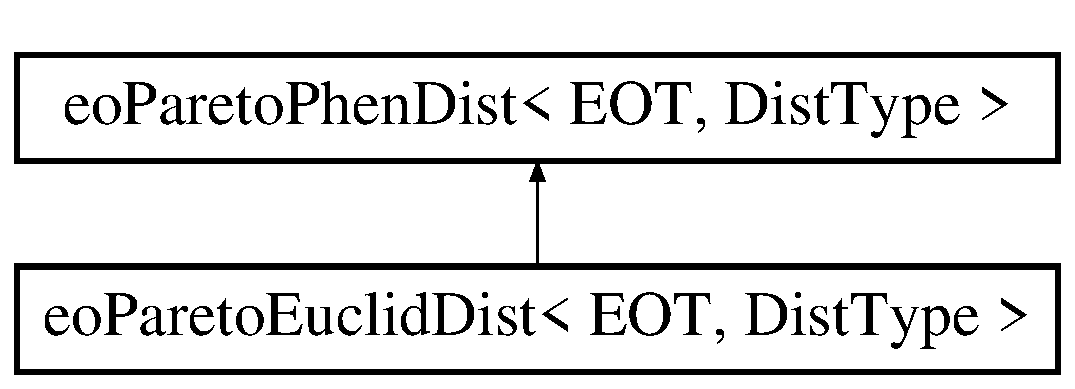
\includegraphics[height=2cm]{classeoParetoEuclidDist}
\end{center}
\end{figure}
\subsection*{Public Member Functions}
\begin{CompactItemize}
\item 
Dist\-Type {\bf operator()} (const EOT \&eopf1, const EOT \&eopf2)\label{classeoParetoEuclidDist_8693ded671292b210c3c455fa18c496e}

\end{CompactItemize}


\subsection{Detailed Description}
\subsubsection*{template$<$class EOT, class Dist\-Type = double$>$ class eo\-Pareto\-Euclid\-Dist$<$ EOT, Dist\-Type $>$}





Definition at line 15 of file eo\-Pareto\-Phen\-Dist.h.

The documentation for this class was generated from the following file:\begin{CompactItemize}
\item 
eo\-Pareto\-Phen\-Dist.h\end{CompactItemize}
